
\documentclass[aspectratio=169]{beamer}
\usetheme{metropolis}
\usefonttheme{professionalfonts}
% !TeX root = raytracing/slides/main.tex
% raytracing_preamble.tex
% Common styling for Ray Tracing presentation

\documentclass[10pt]{beamer}
\usetheme{metropolis}
\usefonttheme{professionalfonts}

% --- Color Definitions ---
\definecolor{PrimaryColor}{RGB}{33,52,72}         % Deep navy
\definecolor{SecondaryColor}{RGB}{84,119,146}     % Desaturated blue-gray
\definecolor{AccentColor}{RGB}{100, 156, 165}       % Soft steel blue

\definecolor{BackgroundColor}{RGB}{245,247,250}   % Very light cool gray/blue-tinted white
\definecolor{TextColor}{RGB}{40,55,70}            % Darker, cool-toned charcoal (slightly less saturated)
\definecolor{LightGray}{RGB}{220,225,230}         % Soft, cool light gray
\definecolor{DarkGray}{RGB}{70,90,105}            % Cool-toned dark gray (coherent with Primary/Secondary)

\definecolor{RayColor}{RGB}{230,150,80}           % Muted warm orange (less saturated than pure orange)
\definecolor{ObjectColor}{RGB}{128,101,160}       % Muted violet (adjusted purple to match cool palette)
\definecolor{LightColor}{RGB}{235,200,100}        % Soft golden yellow (to complement cool blues)

% --- Theme Customization ---
\setbeamercolor{background canvas}{bg=BackgroundColor}
\setbeamercolor{normal text}{fg=TextColor}
\setbeamercolor{frametitle}{bg=PrimaryColor, fg=white}
\setbeamercolor{section in toc}{fg=PrimaryColor}
\setbeamercolor{block title}{bg=PrimaryColor!80, fg=white}
\setbeamercolor{block body}{bg=PrimaryColor!10}
\setbeamercolor{alerted text}{fg=AccentColor}
\setbeamercolor{itemize item}{fg=PrimaryColor}
\setbeamercolor{itemize subitem}{fg=SecondaryColor}
\setbeamerfont{frametitle}{size=\large,series=\bfseries}

% --- Packages ---
\usepackage[utf8]{inputenc}
\usepackage{url}
\usepackage{booktabs}
\usepackage{amsmath, amssymb}
\usepackage{fontawesome5}
\usepackage{pifont}
\usepackage[most]{tcolorbox}
\tcbuselibrary{skins}
\usepackage{colortbl}
\usepackage{array}
\usepackage{tikz}
\usepackage{graphicx}
\usetikzlibrary{shapes.callouts, positioning, arrows.meta, shapes.geometric, shadows, calc, patterns, 3d, backgrounds, shadings}
\usepackage{adjustbox}
\usepackage{ragged2e}
\usepackage{pgfplots}
\usepackage{graphicx}
\usepackage{caption}
\usepackage{minted}
\pgfplotsset{compat=1.18}

% --- Custom Commands ---
\newcommand{\cmark}{\textcolor{SecondaryColor}{\ding{51}}}
\newcommand{\xmark}{\textcolor{AccentColor}{\ding{55}}}
\newcommand{\highlight}[1]{\textcolor{PrimaryColor}{\textbf{#1}}}
\newcommand{\raycolor}[1]{\textcolor{RayColor}{\textbf{#1}}}
\newcommand{\objectcolor}[1]{\textcolor{ObjectColor}{\textbf{#1}}}

% --- TikZ styles for ray tracing visualizations ---
\tikzstyle{process} = [rectangle, rounded corners=3mm, minimum width=2cm, minimum height=0.8cm, text centered, draw=PrimaryColor, thick, fill=PrimaryColor!15, drop shadow]
\tikzstyle{arrow} = [thick, PrimaryColor, ->, >=stealth]
\tikzstyle{ray} = [thick, RayColor, ->, >=stealth]
\tikzstyle{lightray} = [thick, LightColor, ->, >=stealth]
\tikzstyle{reflectray} = [thick, SecondaryColor, ->, >=stealth]
\tikzstyle{refractray} = [thick, AccentColor, ->, >=stealth]
\tikzstyle{shadowray} = [thick, DarkGray, ->, >=stealth, dashed]

% --- 3D object styles ---
\tikzstyle{sphere} = [circle, minimum size=1.5cm, draw=ObjectColor, thick, fill=ObjectColor!20, drop shadow]
\tikzstyle{plane} = [rectangle, minimum width=3cm, minimum height=0.2cm, draw=ObjectColor, thick, fill=ObjectColor!20]
\tikzstyle{triangle} = [regular polygon, regular polygon sides=3, minimum size=1.5cm, draw=ObjectColor, thick, fill=ObjectColor!20]

% --- Eye/Camera styles ---
\tikzstyle{eye} = [circle, minimum size=0.8cm, draw=PrimaryColor, thick, fill=PrimaryColor!30]
\tikzstyle{pixel} = [rectangle, minimum size=0.2cm, draw=AccentColor, fill=AccentColor!30]

% --- Text box styles ---
\tikzstyle{conceptbox} = [rectangle, rounded corners, fill=PrimaryColor!10, draw=PrimaryColor, thick, text width=0.8\textwidth, inner sep=8pt]
\tikzstyle{formulabox} = [rectangle, rounded corners, fill=SecondaryColor!10, draw=SecondaryColor, thick, inner sep=6pt]

% --- Custom environments ---
\newtcolorbox{raybox}[1]{
  colback=RayColor!10,
  colframe=RayColor,
  title=#1,
  fonttitle=\bfseries,
  sharp corners
}

\newtcolorbox{conceptbox}[1]{
  colback=PrimaryColor!10,
  colframe=PrimaryColor,
  title=#1,
  fonttitle=\bfseries,
  rounded corners
}

\newtcolorbox{mathbox}[1]{
  colback=SecondaryColor!10,
  colframe=SecondaryColor,
  title=#1,
  fonttitle=\bfseries,
  rounded corners
}

\newenvironment{timeline}{%
  \begin{tikzpicture}[scale=0.8]
    \coordinate (start) at (0,0);
    \newcounter{timelineitem}
    \setcounter{timelineitem}{0}
  }{%
  \end{tikzpicture}
}

\newcommand{\timelineitem}[4]{%
  \stepcounter{timelineitem}%
  % Name of this item’s node
  \edef\thisID{time\thetimelineitem}%
  \ifnum\value{timelineitem}=1
  % First item: anchor at (start)
  \node[rectangle, draw, fill=PrimaryColor!20,
  text width=1.5cm, minimum height=0.8cm, align=center]
  (\thisID) at (start) {\textbf{#2}};
  \else
  % Later items: below=#1 of previous time node
  \pgfmathtruncatemacro\prev{\value{timelineitem}-1}%
  \node[rectangle, draw, fill=PrimaryColor!20,
    text width=1.5cm, minimum height=0.8cm, align=center,
  below=#1 of time\prev]
  (\thisID) {\textbf{#2}};
  \fi
  % Description always to the right of this time node
  \node[rectangle, draw, fill=SecondaryColor!10,
    text width=4cm, minimum height=0.8cm,
  align=left, right=0.3cm of \thisID]
  (desc\thetimelineitem) {\textbf{#3}\\#4};
  % Draw arrow back to previous if not the first
  \ifnum\value{timelineitem}>1
  \draw[->, thick, PrimaryColor]
  (time\prev.south) -- (\thisID.north);
  \fi
}

\tikzset{
  camera/.style={fill=PrimaryColor!60, draw=PrimaryColor!80, rectangle, minimum size=8pt},
  image plane/.style={fill=AccentColor!10, draw=AccentColor!50, opacity=0.8},
  pixel/.style={fill=AccentColor!60, thick},
  primary ray/.style={->, very thick, red!90},
  object/.style={fill=ObjectColor!60, draw=ObjectColor!80, circle, minimum size=12pt},
  fovangle/.style={<->, thick, PrimaryColor, dashed}
}

\tikzset{
  lens/.style={thick, PrimaryColor, line width=3pt},
  focal plane/.style={thick, AccentColor},
  object ray/.style={->, thick, ObjectColor},
  image ray/.style={->, thick, SecondaryColor},
  optical axis/.style={dashed, gray}
}

\newcommand{\lens}[3]{%
  \begingroup
  % half‐dimensions
  \pgfmathsetlengthmacro{\a}{#2}%
  \pgfmathsetlengthmacro{\b}{#3}%
  \pgfmathsetlengthmacro{\c}{#3/2}%
  \begin{scope}[shift={#1}]
    \draw[line join=round, fill=blue!15]
    (0,-{\c})
    arc(-30:30:{\a} and {\b})
    arc(150:210:{\a} and {\b})
    ;
  \end{scope}
  \endgroup
}


\usepackage{tikz}
\usepackage{pgfplots}
\usepackage{listings}
\usepackage{xcolor}
\usepackage{amsmath}
\usepackage{amssymb}
\usepackage{algorithm2e}
\usepackage{caption}
\usepackage{subcaption}

\usetikzlibrary{arrows.meta}
\usetikzlibrary{shapes}
\usetikzlibrary{positioning}
\usetikzlibrary{decorations.pathreplacing}
\usetikzlibrary{patterns}
\usetikzlibrary{calc}

\lstset{
    language=C++,
    basicstyle=\tiny\ttfamily,
    keywordstyle=\color{blue},
    commentstyle=\color{green!50!black},
    stringstyle=\color{red},
    numberstyle=\tiny\color{gray},
    frame=single,
    breaklines=true,
    showstringspaces=false
}

\lstdefinestyle{glslstyle}{
    language=C,
    basicstyle=\tiny\ttfamily,
    keywordstyle=\color{blue!80!black},
    commentstyle=\color{green!60!black},
    stringstyle=\color{red!60!black},
    numbers=left,
    numberstyle=\tiny\color{gray},
    breaklines=true,
    showstringspaces=false,
    backgroundcolor=\color{gray!5},
    frame=none,
    tabsize=2,
    captionpos=b
}




\title{Motion Blur using Velocity Buffers}
\subtitle{Graphics Assignment CSE 409}
\author{ Team AmarGraphics \\
2005067 - Masnoon Muztahid \\
2005074 - Dipanta Kumar Roy Nobo \\
2005090 - Tawkir Aziz Rahman}
\institute{Department of Computer Science and Engineering\\ Bangladesh University of Engineering and Technology (BUET)}
\date{\today}

\begin{document}

\begin{frame}
  \titlepage
\end{frame}

\begin{frame}{Introduction to Motion Blur}
    \begin{columns}
        \begin{column}{0.55\textwidth}
            \textbf{What is Motion Blur?}
            \begin{itemize}
                \item Visual artifact from object movement during exposure
                \item Creates streaking effects along motion direction  
                \item Essential for realistic rendering
                \item Conveys speed and movement
                \item Reduces temporal aliasing
            \end{itemize}
            
            \vspace{0.2cm}
            \textbf{Why Important?}
            \begin{itemize}
                \item Human vision expects blur
                \item Fast objects appear choppy without it
                \item Enhances immersion
            \end{itemize}
        \end{column}
        
        \begin{column}{0.45\textwidth}
            \begin{figure}
                \centering
                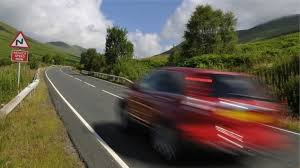
\includegraphics[width=0.8\linewidth]{carSpeedingBlurred.png}
                \caption{Motion Blur}
                \label{fig:placeholder}
            \end{figure}
            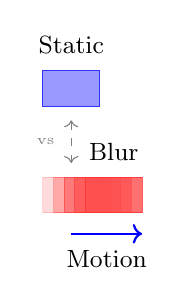
\begin{tikzpicture}[scale=0.9]
                
                \draw[fill=blue!40, draw=blue!80] (0,2.5) rectangle (0.8,3);
                \node[above, font=\small] at (0.4,3.1) {Static};
                
                
                \foreach \i/\op in {0/0.2, 0.15/0.35, 0.3/0.5, 0.45/0.65, 0.6/0.8} {
                    \draw[fill=red!\op!red!70, draw=red!80, opacity=\op] 
                         (\i,1) rectangle (\i+0.8,1.5);
                }
                
                \draw[->, thick, blue] (0.4,0.7) -- (1.4,0.7);
                \node[below, font=\small] at (0.9,0.6) {Motion};
                \node[above, font=\small] at (1,1.6) {Blur};
                

            
                \draw[<->, gray, dashed] (0.4,2.3) -- (0.4,1.7);
                \node[left, font=\tiny, gray] at (0.3,2) {vs};
            \end{tikzpicture}
        \end{column}
    \end{columns}
\end{frame}


\begin{frame}{Real-World vs. CG Motion Blur}
    \begin{columns}[t]
        \begin{column}{0.48\textwidth}
            \textbf{Real-World Motion Blur}
            \begin{itemize}
                \item[\textcolor{green}{\checkmark}] Natural phenomenon
                \item[\textcolor{green}{\checkmark}] Finite shutter speed
                \item[\textcolor{green}{\checkmark}] Continuous exposure
                \item[\textcolor{red}{\times}] No post-control
                \item[\textcolor{red}{\times}] May be unwanted
            \end{itemize}
            
            \vspace{0.2cm}
            \hspace{1cm}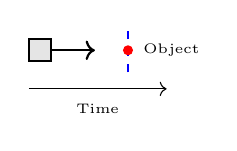
\begin{tikzpicture}[scale=0.7]
                
                \draw[thick, fill=gray!20] (0,1) rectangle (0.4,1.4);
                \draw[->, thick] (0.4,1.2) -- (1.2,1.2);
                
                
                \draw[dashed, blue] (1.8,0.8) -- (1.8,1.6);
                \filldraw[red] (1.8,1.2) circle (0.08);
                \node[right, font=\tiny] at (1.9,1.2) {Object};
                
                
                \draw[->] (0,0.5) -- (2.5,0.5);
                \node[below, font=\tiny] at (1.25,0.4) {Time};
            \end{tikzpicture}
        \end{column}
        
        \begin{column}{0.48\textwidth}
            \textbf{CG Motion Blur}
            \begin{itemize}
                \item[\textcolor{green}{\checkmark}] Precise control
                \item[\textcolor{green}{\checkmark}] Adjustable amount
                \item[\textcolor{green}{\checkmark}] Selective application  
                \item[\textcolor{red}{\times}] Computationally heavy
                \item[\textcolor{red}{\times}] Needs special techniques
            \end{itemize}
            
            \vspace{0.2cm}
            \hspace{1cm}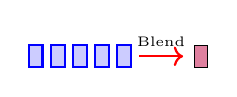
\begin{tikzpicture}[scale=0.7]
                
                \foreach \x in {0,0.4,0.8,1.2,1.6} {
                    \draw[thick, blue, fill=blue!20] (\x,0.8) rectangle (\x+0.25,1.2);
                }
                
               
                \draw[->, thick, red] (2,1) -- (2.8,1);
                \node[above, font=\tiny] at (2.4,1) {Blend};
                
                
                \draw[fill=purple!50] (3,0.8) rectangle (3.25,1.2);
            \end{tikzpicture}
        \end{column}
    \end{columns}
    
    \vspace{0.4cm}
    \begin{center}
        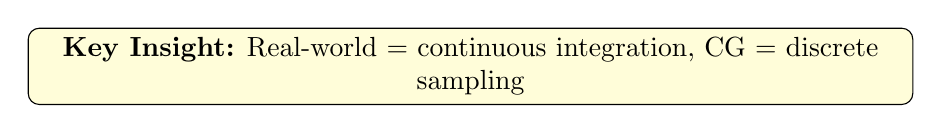
\begin{tikzpicture}
            \node[draw, rounded corners, fill=yellow!15] at (0,0) {
                \parbox{11cm}{\centering \textbf{Key Insight:} Real-world = continuous integration, CG = discrete sampling}
            };
        \end{tikzpicture}
    \end{center}
\end{frame}



\begin{frame}{Types of Motion Blur}
    \begin{tikzpicture}[
        box/.style={draw, rounded corners, fill=blue!15, minimum width=2.2cm, minimum height=1.2cm},
        arrow/.style={->, thick, blue}
    ]
        
        \node[font=\Large\bfseries] at (6,7.5) {Motion Blur Types};
        
        \node[box] (obj) at (2,6) {\textbf{Object\\Motion}};
        \node[below=0.05cm of obj, font=\tiny, text width=2cm, align=center] {Moving objects};
        
        \node[box] (cam) at (6,6) {\textbf{Camera\\Motion}};
        \node[below=0.05cm of cam, font=\tiny, text width=2cm, align=center] {Moving camera};
        
        \node[box] (def) at (10,6) {\textbf{Deformation\\Blur}};
        \node[below=0.05cm of def, font=\tiny, text width=2cm, align=center] {Shape changes};
        
        \begin{scope}[shift={(2,4.5)}]
            \foreach \i/\op in {0/1, 0.2/0.7, 0.4/0.4, 0.6/0.2} {
                \draw[fill=red!\op!red, opacity=\op] (\i,0) circle (0.12);
            }
            \draw[->, blue] (0,-0.3) -- (0.8,-0.3);
        \end{scope}
         
        \begin{scope}[shift={(6,4.5)}]
            \draw[dashed, gray] (0,0) -- (0.8,0.3);
            \draw[dashed, gray] (0,0) -- (0.8,0);
            \draw[dashed, gray] (0,0) -- (0.8,-0.3);
            \filldraw[blue] (0,0) circle (0.04);
            \node[right, font=\tiny] at (0.9,0) {Scene};
        \end{scope}
        
        \begin{scope}[shift={(10,4.5)}]
            \draw[blue, thick] (0,0) sin (0.3,0.2) cos (0.6,0);
            \draw[red, opacity=0.6] (0,0) sin (0.25,0.25) cos (0.5,0);
            \draw[green, opacity=0.6] (0,0) sin (0.35,0.15) cos (0.7,0);
        \end{scope}
        
        \node[draw, rounded corners, fill=green!10] at (6,2.5) {
            \parbox{10cm}{
                \textbf{Implementation Techniques:}\\[0.1cm]
                \begin{columns}
                    \hspace{0.5cm}\begin{column}{0.5\textwidth}
                        • Multi-sampling (accumulation)\\
                        • Velocity buffers \textbf{(our focus)}
                    \end{column}
                    \begin{column}{0.5\textwidth}
                        • Post-process filters\\
                        • Per-pixel motion vectors
                    \end{column}
                \end{columns}
            }
        };
    \end{tikzpicture}
\end{frame}


\begin{frame}{What is a Velocity Buffer?}
    \begin{columns}[t]
        \begin{column}{0.58\textwidth}
            \textbf{Definition:}
            \begin{itemize}
                \item Render target with per-pixel velocity vectors
                \item Encodes 2D screen-space motion  
                \item RG channels store x,y velocity
                \item Enables post-process motion blur
            \end{itemize}
            
            \vspace{0.2cm}
            \textbf{Advantages:}
            \begin{itemize}
                \item[\textcolor{green}{\checkmark}] Single geometry pass
                \item[\textcolor{green}{\checkmark}] Efficient post-processing
                \item[\textcolor{green}{\checkmark}] Quality control
                \item[\textcolor{green}{\checkmark}] Deferred rendering compatible
            \end{itemize}
            
            \vspace{0.2cm}
            
        \end{column}
        
        \begin{column}{0.42\textwidth}
        
            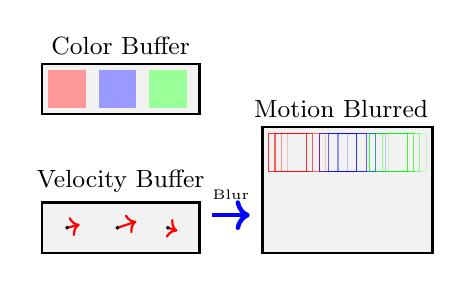
\begin{tikzpicture}[scale=0.8]
                
                \draw[thick, fill=gray!10] (0,3.2) rectangle (2.5,4);
                \node[above, font=\small] at (1.25,4) {Color Buffer};
                \fill[red!40] (0.1,3.3) rectangle (0.7,3.9);
                \fill[blue!40] (0.9,3.3) rectangle (1.5,3.9);
                \fill[green!40] (1.7,3.3) rectangle (2.3,3.9);
                \vspace{1cm}
                
                
                \draw[thick, fill=gray!10] (0,1) rectangle (2.5,1.8);
                \node[above, font=\small] at (1.25,1.8) {Velocity Buffer};
                
                \foreach \x/\dx/\dy in {0.4/0.2/0.05, 1.2/0.3/0.1, 2/0.15/-0.05} {
                    \draw[->, thick, red] (\x,1.4) -- (\x+\dx,1.4+\dy);
                    \filldraw[black] (\x,1.4) circle (0.02);
                }
                
                \draw[->, ultra thick, blue] (2.7,1.6) -- (3.3,1.6);
                \node[above, font=\tiny] at (3,1.7) {Blur};
                
                \draw[thick, fill=gray!10] (3.5,1) rectangle (6.2,3);
                \node[above, font=\small] at (4.75,3) {Motion Blurred};
                
                \foreach \i/\op in {0/0.8, 0.1/0.6, 0.2/0.4, 0.3/0.2} {
                    \draw[red, opacity=\op] (3.6+\i,2.3) rectangle (4.2+\i,2.9);
                    \draw[blue, opacity=\op] (4.4+1.5*\i,2.3) rectangle (5+1.5*\i,2.9);
                    \draw[green, opacity=\op] (5.2+\i,2.3) rectangle (5.8+\i,2.9);
                }
            \end{tikzpicture}
          
            \textbf{Storage (RGBA):}
            \begin{itemize}
                \item \textcolor{red}{R}: Horizontal velocity
                \item \textcolor{green}{G}: Vertical velocity  
                \item \textcolor{blue}{B}: Depth/unused
                \item \textcolor{gray}{A}: Blur mask
            \end{itemize}
        \end{column}
    \end{columns}
\end{frame}


\begin{frame}[fragile,shrink=2]{How Velocity Buffers Are Computed}
    
    \begin{columns}[t]
        \begin{column}{0.36\textwidth} 
            \textbf{Step 1: Vertex Shader}
            \begin{lstlisting}[style=glslstyle, basicstyle=\tiny\ttfamily, numbers=none, backgroundcolor=\color{blue!8}, frame=single]
layout(location = 0) in vec3 position;
uniform mat4 currentMVP, previousMVP;
out vec4 currentPos, previousPos;

void main() {
    vec4 worldPos = vec4(position, 1.0);
    currentPos = currentMVP * worldPos;
    previousPos = previousMVP * worldPos;
    gl_Position = currentPos;
}
            \end{lstlisting}
        \end{column}
        
        \begin{column}{0.30\textwidth}  
            \textbf{Step 2: Fragment Shader}
            \begin{lstlisting}[style=glslstyle, basicstyle=\tiny\ttfamily, numbers=none, backgroundcolor=\color{green!8}, frame=single]
in vec4 currentPos, previousPos;
uniform vec2 screenSize;  
out vec2 velocity;

void main() {
    vec2 currNDC = currentPos.xy / currentPos.w;
    vec2 prevNDC = previousPos.xy / previousPos.w;
    vec2 currScreen = (currNDC * 0.5 + 0.5) * screenSize;
    vec2 prevScreen = (prevNDC * 0.5 + 0.5) * screenSize;
    velocity = currScreen - prevScreen;
}
            \end{lstlisting}
        \end{column}
        
        \begin{column}{0.36\textwidth} 
            \textbf{\scriptsize Mathematical Example:}
            \vspace{0.1cm}
            {\scriptsize
            \begin{align*}
                \text{currNDC} &= (0.2, 0.1) \\
                \text{prevNDC} &= (0.0, 0.0) \\
                \text{screenSize} &= (1920, 1080) \\[0.05cm]
                \text{currScreen} &= (0.2 \times 0.5 + 0.5) \times 1920 = 1152 \\
                &\quad (0.1 \times 0.5 + 0.5) \times 1080 = 594 \\[0.05cm]
                \text{prevScreen} &= (0.0 \times 0.5 + 0.5) \times 1920 = 960 \\
                &\quad (0.0 \times 0.5 + 0.5) \times 1080 = 540 \\[0.05cm]
                \text{velocity} &= (1152, 594) - (960, 540) \\
                &= (192, 54) \text{ pixels}
            \end{align*}
            }
        \end{column}
    \end{columns}
    
    \vspace{0.3cm}
    
    \begin{center}
        \colorbox{yellow!15}{\parbox{12cm}{\centering\Large
            \textbf{Core Idea:} Use current \& previous transforms to compute screen-space motion vectors
        }}
    \end{center}
    
\end{frame}


\begin{frame}[shrink=5]{Velocity Buffer Computation Pipeline}
    
    \begin{center}
        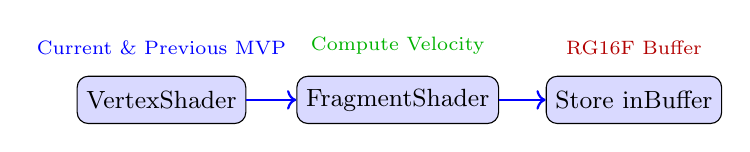
\begin{tikzpicture}[
            box/.style={draw, rounded corners, fill=blue!15, minimum width=1.8cm, minimum height=0.6cm, font=\small},
            arrow/.style={->, thick, blue}
        ]
            \node[box] (vertex) at (0,0) {Vertex\\Shader};
            \node[box] (fragment) at (3,0) {Fragment\\Shader};
            \node[box] (store) at (6,0) {Store in\\Buffer};
            
            \draw[arrow] (vertex) -- (fragment);
            \draw[arrow] (fragment) -- (store);
            
            \node[above=0.15cm of vertex, font=\scriptsize, text=blue] {Current \& Previous MVP};
            \node[above=0.15cm of fragment, font=\scriptsize, text=green!70!black] {Compute Velocity};
            \node[above=0.15cm of store, font=\scriptsize, text=red!70!black] {RG16F Buffer};
        \end{tikzpicture}
    \end{center}
    
    \vspace{0.1cm}
    
    \begin{columns}[t]
        \begin{column}{0.33\textwidth}
            \begin{block}{\textbf{Mathematical Formulation}}
                {\scriptsize
                $P_{curr} = MVP_{curr} \times P_{world}$\\[0.05cm]
                $P_{prev} = MVP_{prev} \times P_{world}$\\[0.05cm]
                $NDC = P.xy/P.w$\\[0.05cm]
                $Screen = (NDC \times 0.5 + 0.5) \times Size$\\[0.05cm]
                $V = Screen_{curr} - Screen_{prev}$
                }
            \end{block}
        \end{column}
        
        \begin{column}{0.33\textwidth}
            \begin{block}{\textbf{Special Considerations}}
                {\scriptsize
                \begin{itemize}
                    \item First frame: velocity = 0
                    \item Camera motion: uniform pixel velocity
                    \item Clamp extreme velocities
                \end{itemize}
                }
            \end{block}
        \end{column}
        
        \begin{column}{0.33\textwidth}
            \begin{block}{\textbf{Buffer Details}}
                {\scriptsize
                \textbf{Format:} RG16F\\[0.1cm]
                \textbf{Channels:} R=horizontal, G=vertical\\[0.1cm]
                \textbf{Range:} ±1024 pixels
                }
            \end{block}
        \end{column}
    \end{columns}
    
    \vspace{0.1cm}
    
    \begin{center}
        \colorbox{yellow!20}{\parbox{9cm}{\centering\small
            \textbf{Pipeline Summary:} Transform vertices with both current and previous MVP matrices, compute screen-space motion vectors in fragment shader, store as velocity buffer
        }}
    \end{center}
    
\end{frame}



\begin{frame}[fragile,shrink=12]{Applying Blur Using the Buffer}
    \begin{columns}[t]
        \begin{column}{0.44\textwidth}
            \textbf{Motion Blur Shader:}
            \begin{lstlisting}[language=GLSL, basicstyle=\tiny\ttfamily, numbers=none, backgroundcolor=\color{blue!8}, frame=single]
// Post-process motion blur
uniform sampler2D colorTexture, velocityTexture;
uniform float blurScale; uniform int maxSamples;
in vec2 texCoord; out vec4 fragColor;

void main() {
    vec2 velocity = texture(velocityTexture, 
        texCoord).xy * blurScale;
    float speed = length(velocity);
    
    if (speed < 0.5) { 
        fragColor = texture(colorTexture, texCoord); 
        return; 
    }
    
    velocity = normalize(velocity) * min(speed, 20.0);
    vec3 result = vec3(0.0);
    
    for (int i = 0; i < maxSamples; ++i) {
        float t = float(i) / float(maxSamples - 1);
        vec2 coord = texCoord - velocity * t / textureSize(colorTexture, 0);
        result += texture(colorTexture, coord).rgb;
    }
    fragColor = vec4(result / float(maxSamples), 1.0);
}
            \end{lstlisting}
        \end{column}
        
        \begin{column}{0.32\textwidth}
            \textbf{Sampling Strategy:}
            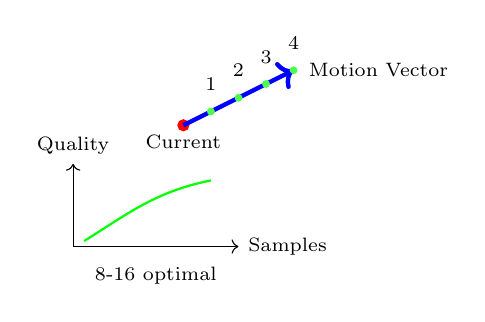
\begin{tikzpicture}[scale=0.7]
                \filldraw[red] (2,2.5) circle (0.1);
                \node[above, font=\scriptsize] at (2,1.9) {Current};
                
                \draw[->, ultra thick, blue] (2,2.5) -- (4,3.5);
                \node[right, font=\scriptsize] at (4.1,3.5) {Motion Vector};
                
                \foreach \i/\t in {1/0.25, 2/0.5, 3/0.75, 4/1.0} {
                    \filldraw[green!70] ($(2,2.5) + \t*(2,1)$) circle (0.06);
                    \node[above, font=\scriptsize] at ($(2,2.5) + \t*(2,1) + (0,0.2)$) {\i};
                }
                
                \begin{scope}[shift={(0,0.3)}]
                    \draw[->] (0,0) -- (3,0) node[right, font=\scriptsize] {Samples};
                    \draw[->] (0,0) -- (0,1.5) node[above, font=\scriptsize] {Quality};
                    \draw[thick, green] (0.2,0.1) .. controls (1,0.6) and (1.5,1) .. (2.5,1.2);
                    \node[below, font=\scriptsize] at (1.5,-0.2) {8-16 optimal};
                \end{scope}
            \end{tikzpicture}
            
            \vspace{0.1cm}
            {\scriptsize
            \textbf{Key Parameters:}
            \begin{itemize}
                \item \textbf{blurScale}: Global intensity (0-2)
                \item \textbf{maxSamples}: Quality (4-32)
                \item \textbf{Velocity clamp}: Max blur (10-50px)
                \item \textbf{Threshold}: Skip static areas
            \end{itemize}
            }
        \end{column}
        
        \begin{column}{0.31\textwidth}
            \vspace{1.2em}
            \begin{tcolorbox}[colback=purple!8, colframe=purple!30, boxrule=0.5pt, arc=2pt, left=1pt, right=1pt, top=1pt, bottom=1pt]
            \textbf{\tiny Color Averaging Example:}
            
            {\tiny
            maxSamples = 4 \\
            velocity = (0.02, 0.01) \\[0.02cm]
            
            Sample 0 (t=0.0): \\
            coord0 = (0.5, 0.5) \\
            color0 = (0.8, 0.2, 0.1) \\[0.02cm]
            
            Sample 1 (t=0.33): \\
            coord1 = (0.493, 0.497) \\
            color1 = (0.6, 0.4, 0.3) \\[0.02cm]
            
            Sample 2 (t=0.67): \\
            coord2 = (0.487, 0.493) \\
            color2 = (0.4, 0.6, 0.5) \\[0.02cm]
            
            Sample 3 (t=1.0): \\
            coord3 = (0.48, 0.49) \\
            color3 = (0.2, 0.8, 0.7) \\[0.02cm]
            
            result = (color0 + color1 \\
            \phantom{result =} + color2 + color3) / 4 \\
            result = (0.5, 0.5, 0.4)
            }
            \end{tcolorbox}
        \end{column}
    \end{columns}
\end{frame}














\begin{frame}{Motion Blur Sampling Strategy}
    \begin{center}
        \textbf{\Large Sampling Along Motion Vector}
    \end{center}
    
    \vspace{0.2cm}
    
    \begin{center}
        
\begin{tikzpicture}[scale=0.75]
            \filldraw[red] (0,1) circle (0.06);
            \node[above, font=\small] at (-2,1.2) {\textbf{Current Pixel}};
            
            \draw[->, ultra thick, blue] (0,1) -- (3,1.5);
            \node[right, font=\small] at (3.1,1.5) {\textbf{Motion Vector}};
            
            \foreach \i/\t in {1/0.2, 2/0.4, 3/0.6, 4/0.8, 5/1.0} {
                \filldraw[green!70] ($(0,1) + \t*(3,0.5)$) circle (0.04);
                \node[above, font=\tiny] at ($(0,1) + \t*(3,0.5) + (0,0.12)$) {S\i};
            }
        \end{tikzpicture}
    \end{center}
    
    \vspace{0.2cm}
    
    \begin{columns}[t]
        \begin{column}{0.32\textwidth}
            \textbf{Sampling Methods:}
            \begin{itemize}
                \item Fixed step
                \item Adaptive
                \item Jittered  
                \item Weighted
            \end{itemize}
            \textbf{Optimal:} 8-16 samples
        \end{column}
        
        \begin{column}{0.33\textwidth}
            \textbf{Sample Weights:}
            \begin{center}
                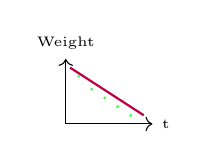
\begin{tikzpicture}[scale=0.55]
                    \draw[->] (0,0) -- (2,0) node[right, font=\tiny] {t};
                    \draw[->] (0,0) -- (0,1.5) node[above, font=\tiny] {Weight};
                    \draw[thick, purple] (0.1,1.3) -- (1.8,0.2);
                    \foreach \i/\t/\w in {1/0.3/1.1, 2/0.6/0.8, 3/0.9/0.6, 4/1.2/0.4, 5/1.5/0.2} {
                        \filldraw[green!70] (\t,\w) circle (0.02);
                    }
                \end{tikzpicture}
            \end{center}
        \end{column}
        
        \begin{column}{0.32\textwidth}
            \textbf{Quality vs Performance:}
            \begin{center}
                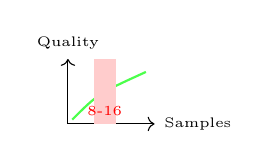
\begin{tikzpicture}[scale=0.55]
                    \draw[->] (0,0) -- (2,0) node[right, font=\tiny] {Samples};
                    \draw[->] (0,0) -- (0,1.5) node[above, font=\tiny] {Quality};
                    \draw[thick, green!70] (0.1,0.1) .. controls (0.7,0.7) .. (1.8,1.2);
                    \fill[red!20] (0.6,0) rectangle (1.1,1.5);
                    \node[font=\tiny, red] at (0.85,0.3) {8-16};
                \end{tikzpicture}
            \end{center}
        \end{column}
    \end{columns}
    
    \vspace{0.3cm}
    
    \begin{center}
        \textbf{Key:} Sample along motion vector with weights decreasing by distance. 
        8-16 samples balance quality and performance.
    \end{center}
\end{frame}



\begin{frame}{Complete Shader Pipeline Overview}
    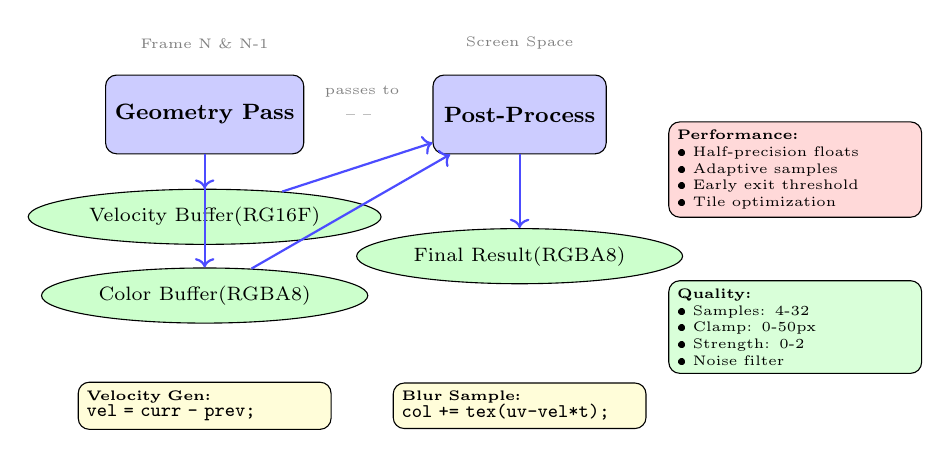
\begin{tikzpicture}[
        stage/.style={draw, rounded corners, fill=blue!20, minimum width=2.2cm, minimum height=1cm, text centered},
        data/.style={draw, ellipse, fill=green!20, minimum width=1.8cm, minimum height=0.7cm, text centered},
        arrow/.style={->, thick, blue!70},
        infobox/.style={draw, rounded corners, fill=#1, text width=3cm, font=\tiny, inner sep=3pt}
    ]
        \node[stage] (geo) at (1.5,5.5) {\footnotesize\textbf{Geometry Pass}};
        \node[data] (vel) at (1.5,4.2) {\scriptsize Velocity Buffer\\(RG16F)};
        \node[data] (color) at (1.5,3.2) {\scriptsize Color Buffer\\(RGBA8)};
        
        \node[stage] (post) at (5.5,5.5) {\footnotesize\textbf{Post-Process}};
        \node[data] (result) at (5.5,3.7) {\scriptsize Final Result\\(RGBA8)};
        
        \draw[arrow] (geo) -- (vel);
        \draw[arrow] (geo) -- (color);
        \draw[arrow] (vel) -- (post);
        \draw[arrow] (color) -- (post);
        \draw[arrow] (post) -- (result);
        
        \node[infobox=yellow!15] (code1) at (1.5,1.8) {
            \textbf{Velocity Gen:}\\
            \texttt{\scriptsize vel = curr - prev;}
        };
        
        \node[infobox=yellow!15] (code2) at (5.5,1.8) {
            \textbf{Blur Sample:}\\
            \texttt{\scriptsize col += tex(uv-vel*t);}
        };
        
        \node[infobox=red!15] (perf) at (9,4.8) {
            \textbf{Performance:}\\
            • Half-precision floats\\
            • Adaptive samples\\
            • Early exit threshold\\
            • Tile optimization
        };
        
        \node[infobox=green!15] (quality) at (9,2.8) {
            \textbf{Quality:}\\
            • Samples: 4-32\\
            • Clamp: 0-50px\\
            • Strength: 0-2\\
            • Noise filter
        };
        
        \node[above=2mm of geo, font=\tiny, gray] {Frame N \& N-1};
        \node[above=2mm of post, font=\tiny, gray] {Screen Space};
        
        \draw[dashed, gray!50] (3.3,5.5) -- (3.7,5.5);
        \node[above, font=\tiny, gray] at (3.5,5.6) {passes to};
        
    \end{tikzpicture}
    
    \vspace{0.3cm}
    
    \begin{center}
        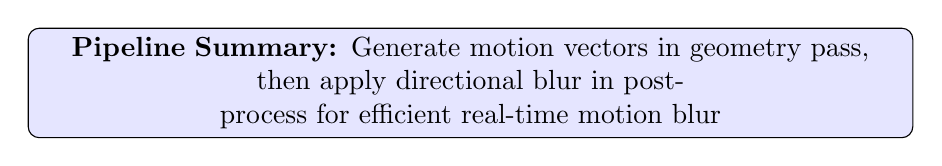
\begin{tikzpicture}
            \node[draw, rounded corners, fill=blue!10, text width=11cm, text centered] {
                \textbf{Pipeline Summary:} Generate motion vectors in geometry pass, \\
                then apply directional blur in post-process for efficient real-time motion blur
            };
        \end{tikzpicture}
    \end{center}
\end{frame}


\begin{frame}{Pros and Cons of Velocity Buffer Motion Blur}
    \begin{columns}[t]
        \begin{column}{0.48\textwidth}
            \textcolor{green}{\large\textbf{ADVANTAGES}}
            \vspace{0.2cm}
            
            \colorbox{green!12}{\parbox{\textwidth-2\fboxsep}{
                \textbf{Performance:}
                \begin{itemize}
                    \item Single geometry pass
                    \item GPU-friendly processing
                    \item No temporal accumulation
                \end{itemize}
                
                \textbf{Quality:}
                \begin{itemize}
                    \item Per-pixel motion vectors
                    \item Controllable blur amount
                    \item Handles complex motion
                \end{itemize}
                
                \textbf{Integration:}
                \begin{itemize}
                    \item Deferred rendering compatible
                    \item Engine-agnostic approach
                    \item Artist-friendly controls
                \end{itemize}
            }}
        \end{column}
        
        \begin{column}{0.48\textwidth}
            \textcolor{red}{\large\textbf{DISADVANTAGES}}
            \vspace{0.2cm}
            
            \colorbox{red!12}{\parbox{\textwidth-2\fboxsep}{
                \textbf{Limitations:}
                \begin{itemize}
                    \item No sub-pixel accuracy
                    \item Occlusion handling issues
                    \item Memory bandwidth cost
                \end{itemize}
                
                \textbf{Artifacts:}
                \begin{itemize}
                    \item Ghosting artifacts
                    \item Edge bleeding
                    \item Velocity discontinuities
                \end{itemize}
                
                \textbf{Implementation:}
                \begin{itemize}
                    \item Needs previous frame data
                    \item Complex animated meshes
                    \item Debug visualization required
                \end{itemize}
            }}
        \end{column}
    \end{columns}
    
    \vspace{0.4cm}
    \begin{center}
        \colorbox{blue!10}{\parbox{0.9\textwidth}{
            \centering
            \textbf{Verdict:} Velocity buffer motion blur is excellent for real-time applications 
            where performance matters more than perfect accuracy. Best suited for games and 
            interactive applications with moderate to high motion.
        }}
    \end{center}
\end{frame}


\begin{frame}{Examples in Real Engines}
    \begin{columns}[t]
        \begin{column}{\textwidth}
            \centering
            \textbf{\Large Motion Blur in Popular Game Engines}
        \end{column}
    \end{columns}
    
    \vspace{0.05cm}
    
    \begin{columns}[t]
        \begin{column}{0.32\textwidth}
            \begin{block}{Unreal Engine}
                \begin{itemize}
                    \item Per-object motion blur
                    \item Temporal upsampling
                    \item TAA integration
                \end{itemize}
            \end{block}
        \end{column}
        
        \begin{column}{0.32\textwidth}
            \begin{block}{Unity HDRP}
                \begin{itemize}
                    \item Camera + object blur
                    \item Quality presets
                    \item VR optimized
                \end{itemize}
            \end{block}
        \end{column}
        
        \begin{column}{0.32\textwidth}
            \begin{block}{CryEngine}
                \begin{itemize}
                    \item Advanced sampling
                    \item Radial blur support
                    \item Dynamic quality
                \end{itemize}
            \end{block}
        \end{column}
    \end{columns}
    
    \vspace{0.05cm}
    
    \begin{block}{Common Implementation Features}
        \begin{columns}[t]
            \begin{column}{0.48\textwidth}
                \begin{itemize}
                    \item Velocity buffer generation
                    \item Post-process blur filter
                    \item Quality/performance settings
                    \item Motion threshold controls
                \end{itemize}
            \end{column}
            \begin{column}{0.48\textwidth}
                \begin{itemize}
                    \item Temporal stability improvements
                    \item VR/mobile optimizations
                    \item Artist-friendly parameters
                    \item Debug visualization tools
                \end{itemize}
            \end{column}
        \end{columns}
    \end{block}
    
    \vspace{0.05cm}
    
    \begin{center}
        \textbf{Quality vs Performance Trade-off:} \\
        \textcolor{blue}{Unity} (High Performance) $\rightarrow$ 
        \textcolor{red}{Unreal} (Balanced) $\rightarrow$ 
        \textcolor{green}{CryEngine} (High Quality)
    \end{center}
\end{frame}


\begin{frame}{Final Thoughts}
    \begin{block}{Key Takeaways}
        \begin{itemize}
            \item \textbf{Velocity buffers} provide an efficient solution for real-time motion blur
            \item \textbf{Single-pass rendering} makes them suitable for modern deferred pipelines
            \item \textbf{Post-process flexibility} allows for quality/performance tuning
            \item \textbf{Wide adoption} in commercial game engines proves their effectiveness
        \end{itemize}
    \end{block}
    
    \vspace{0.3cm}
    
    \begin{columns}[t]
        \begin{column}{0.48\textwidth}
            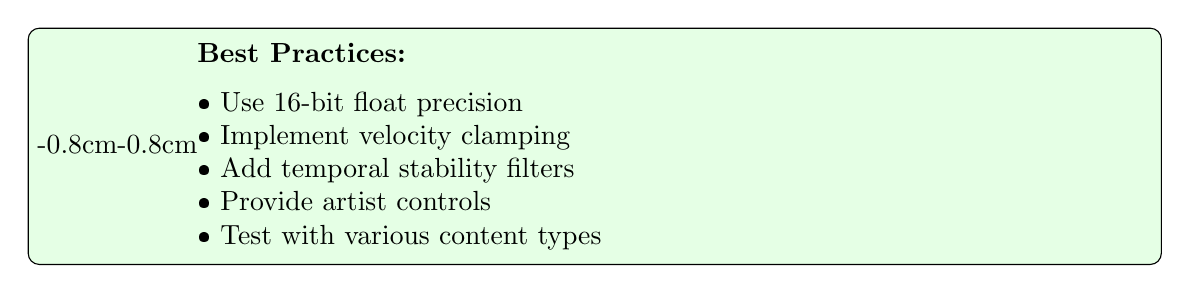
\begin{tikzpicture}
                \node[draw, rounded corners, fill=green!10, minimum width=\textwidth-0.2cm, minimum height=3cm] {
                    \begin{minipage}{\textwidth-0.8cm}
                        \textbf{Best Practices:}\\[0.2cm]
                        • Use 16-bit float precision\\
                        • Implement velocity clamping\\
                        • Add temporal stability filters\\
                        • Provide artist controls\\
                        • Test with various content types
                    \end{minipage}
                };
            \end{tikzpicture}
        \end{column}
        
        \begin{column}{0.48\textwidth}
            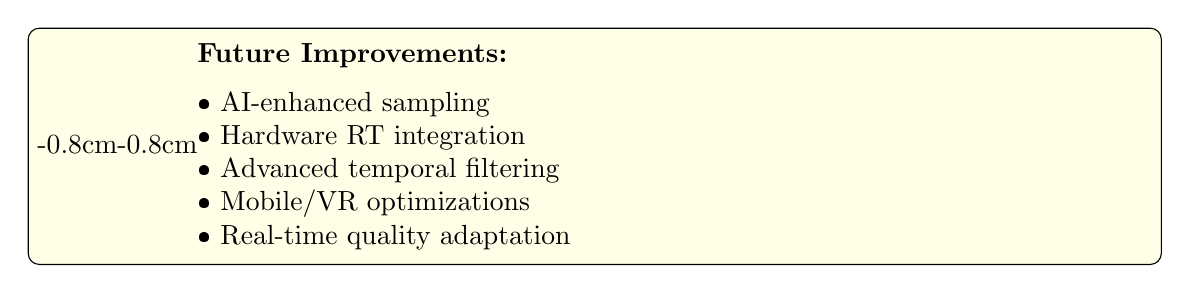
\begin{tikzpicture}
                \node[draw, rounded corners, fill=yellow!10, minimum width=\textwidth-0.2cm, minimum height=3cm] {
                    \begin{minipage}{\textwidth-0.8cm}
                        \textbf{Future Improvements:}\\[0.2cm]
                        • AI-enhanced sampling\\
                        • Hardware RT integration\\
                        • Advanced temporal filtering\\
                        • Mobile/VR optimizations\\
                        • Real-time quality adaptation
                    \end{minipage}
                };
            \end{tikzpicture}
        \end{column}
    \end{columns}
    
    \vspace{0.4cm}
    
    \begin{center}
        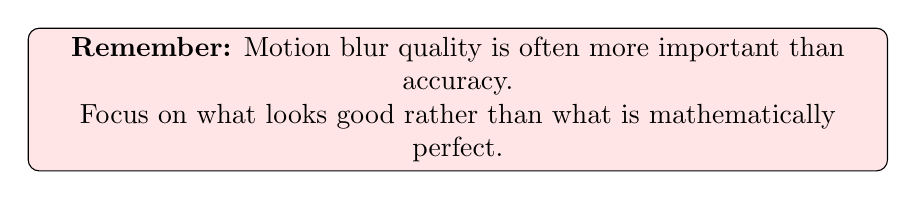
\begin{tikzpicture}
            \node[draw, rounded corners, fill=red!10, minimum width=0.9\textwidth, minimum height=1cm] {
                \begin{minipage}{0.85\textwidth}
                    \centering
                    \textbf{Remember:} Motion blur quality is often more important than accuracy.\\
                    Focus on what looks good rather than what is mathematically perfect.
                \end{minipage}
            };
        \end{tikzpicture}
    \end{center}
    
    \vspace{0.3cm}
    
    \begin{center}
        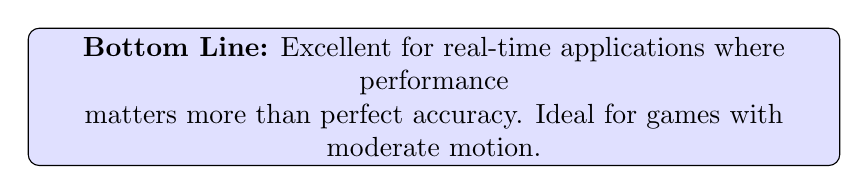
\begin{tikzpicture}
            \node[draw, rounded corners, fill=blue!12, minimum width=0.85\textwidth, minimum height=0.8cm] {
                \begin{minipage}{0.8\textwidth}
                    \centering
                    \textbf{Bottom Line:} Excellent for real-time applications where performance\\
                    matters more than perfect accuracy. Ideal for games with moderate motion.
                \end{minipage}
            };
        \end{tikzpicture}
    \end{center}
\end{frame}



\end{document}